% !TeX root = main.tex

\chapter{随机事件及其概率}
\thispagestyle{plain}

\section{随机事件}

\question 写出下列随机试验的样本空间:

(1)抛一枚硬币,观察正面和反面出现的情况;

(2)抛三枚硬币,观察正面和反面出现的情况;

(3)连续抛一枚硬币,直至出现正面为止;

(4)抛一枚骰子,观察出现的点数;

(5)抛两枚骰子,观察出现的点数;

(6)抛两枚骰子,记录出现的点数之和;

(7)在一个箱子中装有10个同型号的某种零件,其中有3个次品和7个合格品,从该箱子中任取3个零件,观察其中次品的个数;

(8)记录某机场在一天内收到咨询电话的次数;

(9)测试电视机的寿命;

(10)口袋中有黑、白、红球各一个,从中任取两个球;先从中取出一个,放回后再取出一个;

(11)口袋中有黑、白、红球各一个,从中任取两个球;先从中取出一个,不放回后再取出一个.

\begin{solution}
    (1) $\varOmega = \{ 0, 1 \}$,其中 $0$ 表示反面, $1$ 表示正面.

    (2) $\varOmega = \{ (0,0,0), (0,0,1), (0,1,0), (0,1,1), (1,0,0), (1,0,1), (1,1,0), (1,1,1) \}$

    (3) $\varOmega = \{ (1), (0,1), (0,0,1), (0,0,0,1), \cdots \}$

    (4) $\varOmega = \{ 1,2,3,4,5,6 \}$

    (5) $\varOmega = \{ (x,y) \mid x,y = 1,2,3,4,5,6 \}$

    (6) $\varOmega = \{ 2, 3, 4, \cdots, 12 \}$

    (7) $\varOmega = \{ 0,1,2,3 \}$

    (8) $\varOmega = \{ 0,1,2,3,\cdots \}$

    (9) $\varOmega = [0, +\infty)$

    (10) $\varOmega = \{ \text{黑黑}, \text{黑白}, \text{黑红}, \text{白黑}, \text{白白}, \text{白红}, \text{红黑}, \text{红白}, \text{红红} \}$

    (11) $\varOmega = \{ \text{黑白}, \text{黑红}, \text{白黑}, \text{白红}, \text{红黑}, \text{红白} \}$
\end{solution}

\question 设 $A,B,C$ 为三事件,试表示下列事件:

(1) $A$ 发生, $B,C$ 不发生;

(2) $A,B,C$ 都发生;

(3) $A,B,C$ 都不发生;

(4) $A,B,C$ 中只有一个发生;

(5) $A,B,C$ 中至少有一个发生;

(6) $A,B,C$ 中至多有一个发生;

(7) $A,B,C$ 中至少有一个不发生;

(8) $A,B,C$ 中至多有两个发生;

(9) $A,B,C$ 中至少有两个发生;

(10) $A,B,C$ 中恰好有两个发生.

\begin{solution}
    (1) $A \, \overline{B} \, \overline{C}$

    (2) $ABC$

    (3) $\overline{A} \, \overline{B} \, \overline{C}$

    (4) $A \, \overline{B} \, \overline{C} \cup \overline{A} B \overline{C} \cup \overline{A} \, \overline{B} \, C$

    (5) $\varOmega - \overline{A} \, \overline{B} \, \overline{C} = \overline{\overline{A} \, \overline{B} \, \overline{C}} = A \cup B \cup C$

    (6) $\overline{A} \, \overline{B} \, \overline{C} \cup A \, \overline{B} \, \overline{C} \cup \overline{A} B \overline{C} \cup \overline{A} \, \overline{B} \, C$

    (7) $\overline{A} \cup \overline{B} \cup \overline{C}$

    (8) $\varOmega - ABC = \overline{ABC} = \overline{A} \cup \overline{B} \cup \overline{C}$

    (9) $AB \cup AC \cup BC$

    (10) $AB \overline{C} \cup A \overline{B} C \cup \overline{A} BC$
\end{solution}

\question 判断下列命题是否成立:

(1) $A-(B-C) = (A-B) \cup C$;

(2)若 $AB = \text{\O}$ 且 $C \subseteq A$,则 $BC = \text{\O}$;

(3) $(A \cup B) - B = A$;

(4) $(A - B) \cup B = A$.

\begin{solution}
    (1)
    $$
    \begin{aligned}
        A-(B-C) &= A - B \overline{C} \\
        &= A \overline{B \overline{C}} \\
        &= A (\overline{B} \cup C) \\
        &= (A \overline{B}) \cup (AC) \\
        &= (A-B) \cup (AC) \\
        & \not= (A-B) \cup C
    \end{aligned}
    $$
    命题1不成立.

    (2)成立.

    (3)
    $$
    (A \cup B) - B = (A \cup B) \overline{B} = (A \overline{B}) \cup (B \overline{B}) = A \overline{B} \not= A
    $$
    命题3不成立.

    (4)
    $$
    (A - B) \cup B = (A \overline{B}) \cup B = (A \cup B)(\overline{B} \cup B) = A \cup B \not= A
    $$
    命题4不成立.
\end{solution}

\section{随机事件的概率}

\question 设 $A,B$ 是同一个试验中的两个事件, $P(A)=0.6, P(A-B)=0.2, P(A \cup B) = 0.9$.求 $P(\overline{AB}), P(B), P((\overline{A} \cup B)(A \cup \overline{B}))$.

\begin{solution}
    由于 $P(A-B) = P(A) - P(AB)$,所以
    $$
    P(AB) = P(A) - P(A-B) = 0.6 - 0.2 = 0.4
    $$
    进而可得
    $$
    P(\overline{AB}) = 1 - P(AB) = 1 - 0.4 = 0.6
    $$

    由于 $P(A \cup B) = P(A) + P(B) - P(AB)$,所以
    $$
    P(B) = P(A \cup B) - P(A) + P(AB) = 0.9 - 0.6 + 0.4 = 0.7
    $$

    由随机事件的运算性质可得
    $$
    \begin{aligned}
        (\overline{A} \cup B)(A \cup \overline{B}) &= [(\overline{A} \cup B) A] \cup [(\overline{A} \cup B) \overline{B}] \\
        &= (A \overline{A}) \cup (AB) \cup (\overline{A} \, \overline{B}) \cup (B \overline{B}) \\
        &= (AB) \cup (\overline{A \cup B})
    \end{aligned}
    $$
    又因为 $(AB)(\overline{A \cup B}) = (AB)(\overline{A} \, \overline{B}) = \text{\O}$,所以
    $$
    \begin{aligned}
        P((\overline{A} \cup B)(A \cup \overline{B})) &= P((AB) \cup (\overline{A \cup B})) \\
        &= P(AB) + P(\overline{A \cup B}) \\
        &= P(AB) + 1 - P(A \cup B) \\
        &= 0.4 + 1 - 0.9 \\
        &= 0.5
    \end{aligned}
    $$
\end{solution}

\question 设 $A$ 和 $B$ 是同一试验 $E$ 的两个随机事件,证明: $1 - P(\overline{A}) - P(\overline{B}) \leqslant P(AB) \leqslant P(A \cup B)$.

\begin{proof}
    因为 $AB \subseteq A \subseteq (A \cup B)$,所以
    $$
    P(AB) \leqslant P(A \cup B)
    $$

    因为
    $$
    1 - P(AB) = P(\overline{AB}) = P(\overline{A} \cup \overline{B}) \leqslant P(\overline{A}) + P(\overline{B})
    $$
    所以
    $$
    1 - P(\overline{A}) - P(\overline{B}) \leqslant P(AB)
    $$
\end{proof}

\question 已知 $P(A) = P(B) = P(C) = \dfrac{1}{4}, P(AB) = 0, P(AC) = P(BC) = \dfrac{1}{16}$.则 $A,B,C$ 中至少发生一个的概率是多少? $A,B,C$ 都不发生的概率是多少?

\begin{solution}
    因为 $P(AB) = 0$,且 $ABC \subseteq AB$,由概率的单调性可知 $P(ABC) = 0$.由概率的加法公式可得 $A,B,C$ 中至少发生一个的概率为
    $$
    \begin{aligned}
        P(A \cup B \cup C) &= P(A) + P(B) + P(C) - P(AB) - P(BC) - P(AC) + P(ABC) \\
        &= \dfrac{1}{4} + \dfrac{1}{4} + \dfrac{1}{4} - 0 - \dfrac{1}{16} - \dfrac{1}{16} + 0 \\
        &= \dfrac{5}{8}
    \end{aligned}
    $$
    $A,B,C$ 都不发生的概率为
    $$
    \begin{aligned}
        P(\overline{A} \, \overline{B} \, \overline{C}) &= P(\overline{A \cup B \cup C}) \\
        &= 1 - P(A \cup B \cup C) \\
        &= 1 - \dfrac{5}{8} \\
        &= \dfrac{3}{8}
    \end{aligned}
    $$
\end{solution}

\question 抛两枚硬币,求出现一个正面一个反面的概率.

\begin{solution}
    此试验的样本空间为 $\varOmega = \{ (\text{正}, \text{正}), (\text{正}, \text{反}), (\text{反}, \text{正}), (\text{反}, \text{反}) \}$,样本点的个数为4,且每个样本点发生的可能性是相等的.事件``出现一个正面一个反面"含有的样本点个数为2,根据古典概型可得该事件发生的概率为 $\dfrac{1}{2}$.
\end{solution}

\begin{note}
    \indent 如果将样本空间写成 $\varOmega' = \{ (\text{正}, \text{正}), (\text{反}, \text{反}), (\text{一正一反}) \}$,这3个样本点不是等可能的,不满足古典概型的条件.
\end{note}

\question 从 $1,2,\cdots,10$ 这10个数字中任取3个,求大小在中间的数字恰好为5的概率.

\begin{solution}
    从10个数字中任取3个,共有 $\mathrm{C}_{10}^3$ 种取法.如果大小在中间的数字恰好为5,必须有一个小于5、一个等于5、一个大于5,这样的取法有 $\mathrm{C}_4^1 \mathrm{C}_1^1 \mathrm{C}_5^1$ 种.因此所求概率为
    $$
    p = \dfrac{\mathrm{C}_4^1 \mathrm{C}_1^1 \mathrm{C}_5^1}{\mathrm{C}_{10}^3} = \dfrac{4 \times 1 \times 5}{120} = \dfrac{1}{6}
    $$
\end{solution}

\question 任取两个正整数,求它们的和为偶数的概率.

\begin{solution}
    记取出偶数为``0",取出奇数为``1",则随机试验``任取两个正整数"的样本空间为
    $$
    \varOmega = \{ (0,0), (0,1), (1,0), (1,1) \}
    $$
    令事件 $A$ 表示``取出的两个正整数之和为偶数",则 $A = \{ (0,0), (1,1) \}$,从而所求概率为 $$P(A) = \dfrac{1}{2}$$
\end{solution}

\question 将15名新生(其中有3名优秀生)随机地分配到3个班级去,其中一班4名,二班5名,三班6名.求:

(1)每个班级各分配到一名优秀生的概率;

(2) 3名优秀生分配到一个指定班级的概率;

(3) 3名优秀生分配到同一个班级的概率.

\begin{solution}
    将15名新生随机地分配给一班4名、二班5名、三班6名,共有 $\mathrm{C}_{15}^4 \mathrm{C}_{11}^5 \mathrm{C}_6^6$ 种分法.

    (1)将3名优秀生分配到三个班级的分法共有 $\mathrm{A}_3^3$ 种,将其余12名新生分配给一班3名、二班4名、三班5名的分法共有 $\mathrm{C}_{12}^3 \mathrm{C}_9^4 \mathrm{C}_5^5$ 种,则每个班级各分配到一名优秀生的分法共有 $\mathrm{A}_3^3 \mathrm{C}_{12}^3 \mathrm{C}_9^4 \mathrm{C}_5^5$ 种.因此所求概率为
    $$
    p = \dfrac{\mathrm{A}_3^3 \mathrm{C}_{12}^3 \mathrm{C}_9^4 \mathrm{C}_5^5}{\mathrm{C}_{15}^4 \mathrm{C}_{11}^5 \mathrm{C}_6^6} = \dfrac{24}{91}
    $$

    (2)如果将3名优秀生分配到一班,则其余12名新生将分配给一班1名、二班5名、三班6名,此时分法共有 $\mathrm{C}_{12}^1 \mathrm{C}_{11}^5 \mathrm{C}_6^6$ 种,所求概率为
    $$
    p_1 = \dfrac{\mathrm{C}_{12}^1 \mathrm{C}_{11}^5 \mathrm{C}_6^6}{\mathrm{C}_{15}^4 \mathrm{C}_{11}^5 \mathrm{C}_6^6} = \dfrac{4}{455}
    $$

    如果将3名优秀生分配到二班,则其余12名新生将分配给一班4名、二班2名、三班6名,此时分法共有 $\mathrm{C}_{12}^4 \mathrm{C}_{8}^2 \mathrm{C}_6^6$ 种,所求概率为
    $$
    p_2 = \dfrac{\mathrm{C}_{12}^4 \mathrm{C}_{8}^2 \mathrm{C}_6^6}{\mathrm{C}_{15}^4 \mathrm{C}_{11}^5 \mathrm{C}_6^6} = \dfrac{2}{91}
    $$

    如果将3名优秀生分配到三班,则其余12名新生将分配给一班4名、二班5名、三班3名,此时分法共有 $\mathrm{C}_{12}^4 \mathrm{C}_{8}^5 \mathrm{C}_3^3$ 种,所求概率为
    $$
    p_3 = \dfrac{\mathrm{C}_{12}^4 \mathrm{C}_{8}^5 \mathrm{C}_3^3}{\mathrm{C}_{15}^4 \mathrm{C}_{11}^5 \mathrm{C}_6^6} = \dfrac{4}{91}
    $$

    (3)用 $A_i$ 表示``3名优秀生全部分配到 $i$ 班" $(i=1,2,3)$,则事件``3名优秀生分配到同一个班级"可以表示为 $A_1 \cup A_2 \cup A_3$.又因为 $A_i A_j = \text{\O} \, (i \not= j, i,j=1,2,3)$,所以所求概率为
    $$
    p = P(A_1 \cup A_2 \cup A_3) = P(A_1) + P(A_2) + P(A_3) = \dfrac{4}{455} + \dfrac{2}{91} + \dfrac{4}{91} = \dfrac{34}{455}
    $$
\end{solution}

\question 抛两颗骰子,求下列事件的概率:

(1)点数之和为6;

(2)点数之和不超过6;

(3)至少有一个6点.

\begin{solution}
    抛两颗骰子所得点数的样本空间为 $\varOmega = \{ (x,y) \mid x,y=1,2,3,4,5,6 \}$,样本点数量为36.

    (1)令事件 $A$ 为``点数之和为6",则
    $$
    A = \{ (1,5), (2,4), (3,3), (4,2), (5,1) \}
    $$
    所以所求概率为
    $$
    P(A) = \dfrac{5}{36}
    $$

    (2)令事件 $B$ 为``点数之和不超过6",则
    $$
    \begin{aligned}
        B = \{ & (1,1), (1,2), (1,3), (1,4), (1,5), (2,1), (2,2), (2,3), \\
        & (2,4), (3,1), (3,2), (3,3), (4,1), (4,2), (5,1) \}
    \end{aligned}
    $$
    所以所求概率为
    $$
    P(B) = \dfrac{15}{36} = \dfrac{5}{12}
    $$

    (3)令事件 $C$ 为``至少有一个6点",则
    $$
    \begin{aligned}
        C = \{ & (1,6), (2,6), (3,6), (4,6), (5,6), (6,6), \\
        & (6,1), (6,2), (6,3), (6,4), (6,5) \}
    \end{aligned}
    $$
    所以所求概率为
    $$
    P(C) = \dfrac{11}{36}
    $$
\end{solution}

\question 考虑一元二次方程 $x^2 + Bx + C = 0$,其中 $B,C$ 分别是将一颗骰子连续抛两次先后出现的点数,求该方程有实根的概率 $p$ 和有重根的概率 $q$.

\begin{solution}
    将一颗骰子连续抛两次所得点数的样本空间为 $\varOmega = \{ (B,C) \mid B,C=1,2,3,4,5,6 \}$,样本点数量为36.
    
    事件``该方程有实根"发生的条件为 $B^2 - 4C \geqslant 0$,而
    $$
    \begin{aligned}
        \{ B^2 - 4C \geqslant 0 \} = \{ & (2,1), (3,1), (4,1), (5,1), (6,1), (3,2), (4,2), (5,2), (6,2), \\
        & (4,3), (5,3), (6,3), (4,4), (5,4), (6,4), (5,5), (6,5), (5,6), (6,6) \}
    \end{aligned}
    $$
    共有19个样本点,因此
    $$
    p = P(B^2 - 4C \geqslant 0) = \dfrac{19}{36}
    $$

    事件``该方程有重根"发生的条件为 $B^2 - 4C = 0$,而
    $$
    \begin{aligned}
        \{ B^2 - 4C = 0 \} = \{ & (2,1), (4,4) \}
    \end{aligned}
    $$
    共有2个样本点,因此
    $$
    q = P(B^2 - 4C = 0) = \dfrac{2}{36} = \dfrac{1}{18}
    $$
\end{solution}

\question 从 $N$ 个数字 $1,2,\cdots,N$ 中可重复地随机抽取 $n$ 次,求抽到的最大数字正好为 $k \, (1 \leqslant k \leqslant N)$ 的概率.

\begin{solution}
    从 $N$ 个数字中可重复地抽取 $n$ 次,共有 $N^n$ 种取法.

    记事件 $B_i$ 为``抽到的最大数字小于等于 $i$'' ($i=1,2,\cdots,N$),则 $B_i$ 发生只需每次从 $1,2,\cdots,i$ 中取数即可,共有 $i^n$ 种取法,由古典概型可知
    $$
    P(B_i) = \dfrac{i^n}{N^n}
    $$

    记事件 $A_k$ 为``抽到的最大数字正好为 $k$",则 $A_k = B_k - B_{k-1}$,且 $B_{k-1} \subseteq B_k$,因此
    $$
    \begin{aligned}
        P(A_k) &= P(B_k - B_{k-1}) \\
        &= P(B_k) - P(B_{k-1}) \\
        &= \dfrac{k^n}{N^n} - \dfrac{(k-1)^n}{N^n} \\
        &= \dfrac{k^n - (k-1)^n}{N^n}
    \end{aligned}
    $$
\end{solution}

\question 从一副52张的扑克牌中任取4张,求下列事件的概率:

(1)全是黑桃;

(2)同花;

(3)没有两张同一花色;

(4)同色.

\begin{solution}
    从52张扑克牌中任取4张的取法有 $\mathrm{C}_{52}^4$ 种.

    (1)一副扑克牌中有13张黑桃,从中取出4张的取法有 $\mathrm{C}_{13}^4$ 种,因此所求概率为
    $$
    p_1 = \dfrac{\mathrm{C}_{13}^4}{\mathrm{C}_{52}^4} = \dfrac{11}{4165}
    $$

    (2)取出的4张牌全是某一特定花色的取法有 $\mathrm{C}_{13}^4$ 种,而一副扑克牌有4种花色,则4张牌同花的取法有 $4 \mathrm{C}_{13}^4$ 种,因此所求概率为
    $$
    p_2 = \dfrac{4 \mathrm{C}_{13}^4}{\mathrm{C}_{52}^4} = \dfrac{44}{4165}
    $$

    (3)``没有两张同一花色"需要从4种花色中各取一张,取法有 $13^4$ 种,因此所求概率为
    $$
    p_3 = \dfrac{13^4}{\mathrm{C}_{52}^4} = \dfrac{2197}{20825}
    $$

    (4)一副扑克牌中有红色和黑色牌各26张,取出4张同色牌的取法有 $2 \mathrm{C}_{26}^4$ 种,因此所求概率为
    $$
    p_4 = \dfrac{2 \mathrm{C}_{26}^4}{\mathrm{C}_{52}^4} = \dfrac{92}{833}
    $$
\end{solution}

\question 把10本书任意地放在书架上,求其中指定的四本书放在一起的概率.

\begin{solution}
    把10本书任意地放在书架上,共有 $\mathrm{A}_{10}^{10}$ 种放法.当其中指定的四本书放在一起时,将这四本书看作一个整体,与其他6本书一起放在书架上,有 $\mathrm{A}_7^7$ 种放法;放在一起的4本书又有不同的顺序,有 $\mathrm{A}_4^4$ 种放法.因此``其中指定的四本书放在一起''共有 $\mathrm{A}_7^7 \mathrm{A}_4^4$ 种放法,所求概率为
    $$
    p = \dfrac{\mathrm{A}_7^7 \mathrm{A}_4^4}{\mathrm{A}_{10}^{10}} = \dfrac{7! \times 4!}{10!} = \dfrac{1}{30}
    $$
\end{solution}

\question $n$ 个人随机地围一圆桌而坐,求甲、乙两人相邻而坐的概率.

\begin{solution}

    \textbf{解法一:} $n$ 个人围坐,共有 $\dfrac{\mathrm{A}_n^n}{n} = (n-1)!$ 种坐法.当甲、乙两人相邻而坐时,将甲、乙两人看作整体,有 $\dfrac{\mathrm{A}_{n-1}^{n-1}}{n-1} \mathrm{A}_2^2 = 2(n-2)!$ 种坐法.因此所求概率为
    $$
    p = \dfrac{2(n-2)!}{(n-1)!} = \dfrac{2}{n-1}
    $$

    \textbf{解法二:}设甲先坐好,再考虑乙的坐法.此时乙总共有 $n-1$ 个位置可坐,且这 $n-1$ 个位置都是等可能的,而乙与甲相邻有2个位置,因此所求概率为
    $$
    p = \dfrac{2}{n-1}
    $$
\end{solution}

\question 同时掷5枚骰子,求下列事件的概率:

(1)每枚都不一样;

(2)其中2枚相同(成对),另外3枚各不相同且与成对的2枚也不同;

(3)出现两组成对的骰子;

(4)其中3枚相同,另外2枚不同;

(5)其中4枚相同;

(6) 5枚全部相同.

\begin{solution}
    同时掷5枚骰子共有 $6^5$ 种不同情况.

    \vspace{0.3em}

    (1) $p_1 = \dfrac{6 \times 5 \times 4 \times 3 \times 2}{6^5} = \dfrac{5}{54}$

    \vspace{0.3em}

    (2) $p_2 = \dfrac{\mathrm{C}_5^2 \times 6 \times 5 \times 4 \times 3}{6^5} = \dfrac{25}{54}$

    \vspace{0.3em}

    (3)将5枚骰子分成3组,其中2组包含2枚骰子,另外一组只有1个骰子,这样的分法有 $\dfrac{\mathrm{C}_5^2 \mathrm{C}_3^2}{2} = 15$ 种.这三组骰子出现的点数不同,有 $6 \times 5 \times 4 = 120$ 种情况,因此所求概率为
    $$
    p_3 = \dfrac{15 \times 120}{6^5} = \dfrac{25}{108}
    $$

    (4) $p_4 = \dfrac{\mathrm{C}_5^3 \times 6 \times 5 \times 4}{6^5} = \dfrac{25}{162}$

    \vspace{0.3em}

    (5) $p_5 = \dfrac{\mathrm{C}_5^4 \times 6 \times 5}{6^5} = \dfrac{25}{1296}$

    (6) $p_6 = \dfrac{6}{6^5} = \dfrac{1}{1296}$
\end{solution}

\question 在长度为 $a$ 的线段内任取两点将其分为三段,求它们可以构成一个三角形的概率.

\begin{solution}
    设分成的三段长度分别为 $x, y$ 和 $a-x-y$,则有
    $$
    \begin{cases}
        0<x<a \\
        0<y<a \\
        0 < a-x-y < a
    \end{cases}
    $$
    其中 $0 < a-x-y < a$ 等价于 $0 < x+y < a$,则样本空间为
    $$
    \varOmega = \{ (x,y) \mid 0<x<a,\ 0<y<a,\ 0 < x+y < a \}
    $$

    设事件 $A = \text{``线段分成的三段可以构成三角形"}$.由于三角形中任意两边之和大于第三边,则事件 $A$ 发生的条件为
    $$
    \begin{cases}
        0 < x < y + (a-x-y) \\
        0 < y < x + (a-x-y) \\
        0 < a-x-y < x+y
    \end{cases}
    $$
    整理得
    $$
    A = \{ (x,y) \mid 0 < x < \dfrac{a}{2},\ 0 < y < \dfrac{a}{2},\ \dfrac{a}{2} < x+y < a \}
    $$
    如图 \ref{fig:example-三角形} 所示.则所求概率为
    $$
    P(A) = \dfrac{\dfrac{1}{2} \left( \dfrac{a}{2} \right)^2}{\dfrac{1}{2} a^2} = \dfrac{1}{4}
    $$

    \begin{figure}[H]
        \centering

        \begin{tikzpicture}[scale=1.1]
            % 坐标轴
            \draw[->] (-0.5, 0)--(3.5, 0) node[below]{$x$};
            \draw[->] (0, -0.5)--(0, 3.5) node[left]{$y$};
            \node at (0, 0) [below left] {$O$};
            % 定义特殊点
            \coordinate (A) at (0, 3);
            \coordinate (B) at (3, 0);
            \coordinate (C) at (0, 1.5);
            \coordinate (D) at (1.5, 0);
            \coordinate (E) at (1.5, 1.5);
            % 曲线
            \draw (A) node[left]{$a$} -- (B) node[below]{$a$};
            \draw (C) node[left]{$\dfrac{a}{2}$} -- (D) node[below]{$\dfrac{a}{2}$} -- (E) -- cycle;
            % 填充
            \filldraw[fill=lightgray] (C) -- (D) -- (E) -- cycle;
            % 区域标记
            \node at (1,1) {$A$};
            \node at (0.5, 2) {$\varOmega$};
        \end{tikzpicture}
        
        \caption{}
        \label{fig:example-三角形}
    \end{figure}
\end{solution}